% Векторизация циклов с нерегулярным количеством итераций.
\subsection{Векторизация гнезд циклов с нерегулярным количеством итераций}

Сортировка Шелла [13] представляет собой расширение сортировки вставками, которое работает быстрее, так как позволяет на ранних этапах упорядочить далеко расположенные друг от друга элементы массива, это приводит к тому, что массив становится частично упорядоченным.
Во время сортировки Шелла выполняется последовательная сортировка подмассивов основного массива, являющихся срезами, при этом шаг среза постоянно уменьшается и на завершающем этапе выполняется обычная сортировка вставками (это соответствует срезу массива с шагом 1).
Выполнение сортировки срезов массива с большими шагами облегчает сортировку срезов с меньшими значениями шага, эффективность сортировки существенно зависит от выбранной последовательности шагов.

В литературе описано множество существующих последовательностей, из которых мы будем анализировать лишь представленные в таблице 1 [14–16]:

\begin{center}
\begin{tabular}{ | c | c | }
  \hline
  Последовательность & Формула \\ \hline
  \makecell{Последовательность Шелла, 1959 г.} & \makecell{$k_1 = \lfloor \frac{N}{2} \rfloor$, $k_i = \lfloor \frac{k_i - 1}{2} \rfloor$, $k_t = 1$} \\ \hline
  \makecell{Последовательность Хиббарда, 1963 г.} & \makecell{$2^i - 1 \le N$, $i \in \mathbb{N}$} \\ \hline
  \makecell{Последовательность Пратта, 1971 г.} & \makecell{$2^i \cdot 3^j \le \frac{N}{2}$, $i \in \mathbb{N}$, $j \in \mathbb{N}$} \\ \hline
  \makecell{Последовательность Седжвика, 1986 г.} & \makecell{$k_i = \begin{cases} 9 \cdot 2^i - 9 \cdot 2^{\frac{i}{2}} + 1, \ k even \\ 8 \cdot 2^i - 6 \cdot 2^{\frac{i + 1}{2}}, k \ odd \end{cases}$} \\ \hline
\end{tabular}
\end{center}

Каноническая реализация сортировки Шелла состоит из гнезда циклов, содержащего три цикла. Внешний цикл выполняется по всем шагам из используемой последовательности шагов, начиная с максимального и заканчивая единицей.
Два внутренних цикла осуществляют сортировку всех подмассивов, являющихся срезами исходного массива с текущим шагом k (рисунок 1).

\begin{figure}[ht]
	\centering
		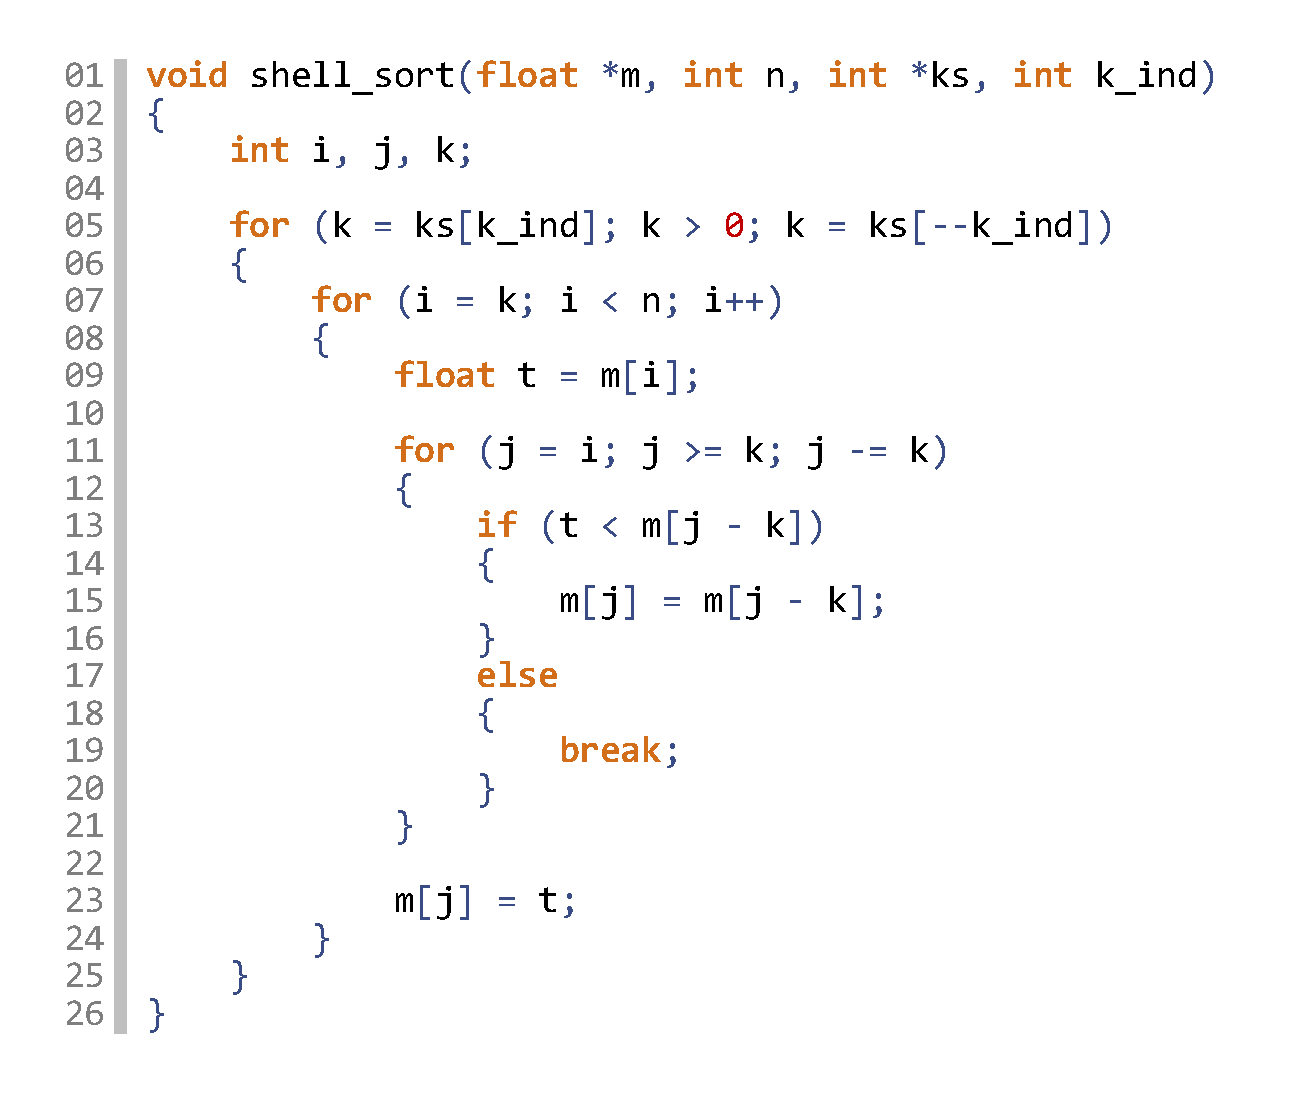
\includegraphics[width=0.8\textwidth]{./pics/text_4_vec_irreg/shell_code.pdf}
	\caption{}
	\label{fig:text_4_vec_irreg_shell_code}
\end{figure}

\begin{figure}[ht]
	\centering
		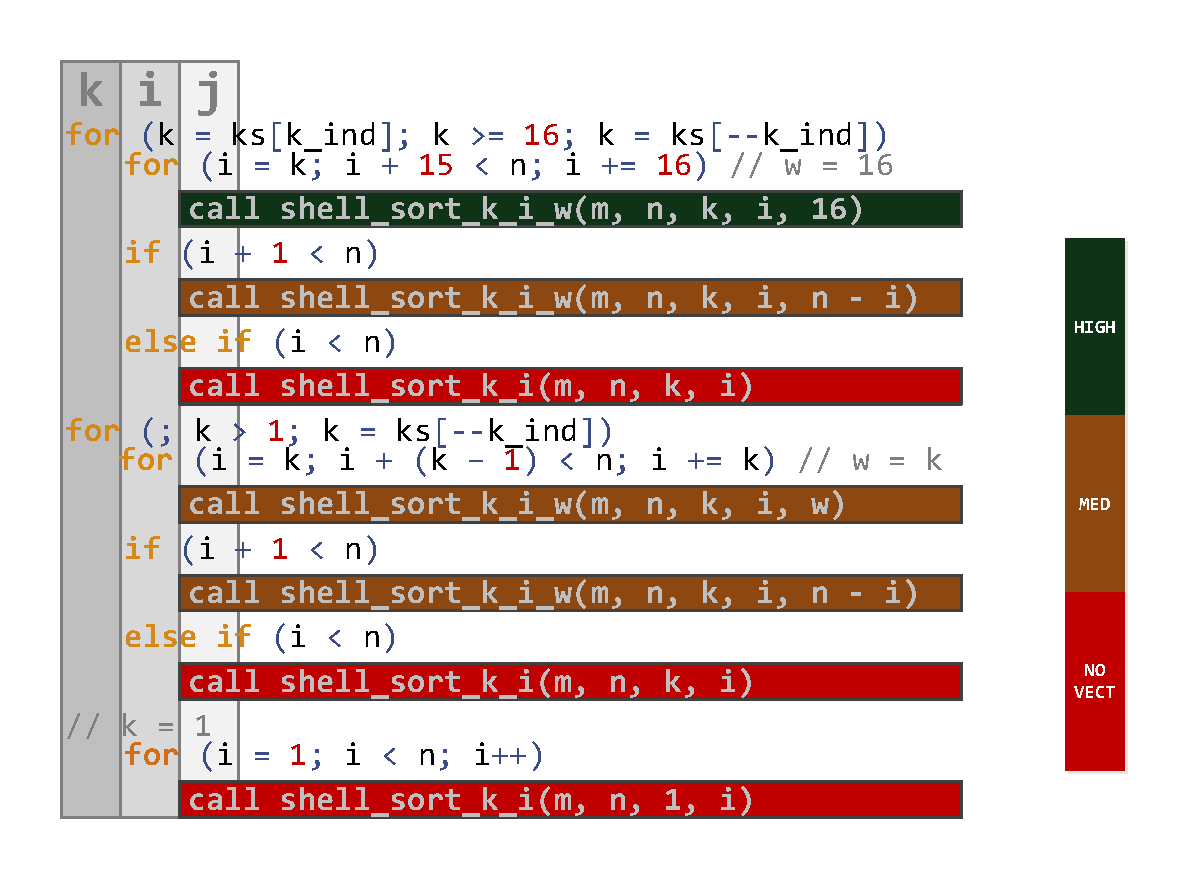
\includegraphics[width=0.8\textwidth]{./pics/text_4_vec_irreg/code_decomp.pdf}
	\caption{}
	\label{fig:text_4_vec_irreg_code_decomp}
\end{figure}

\begin{figure}[ht]
	\centering
		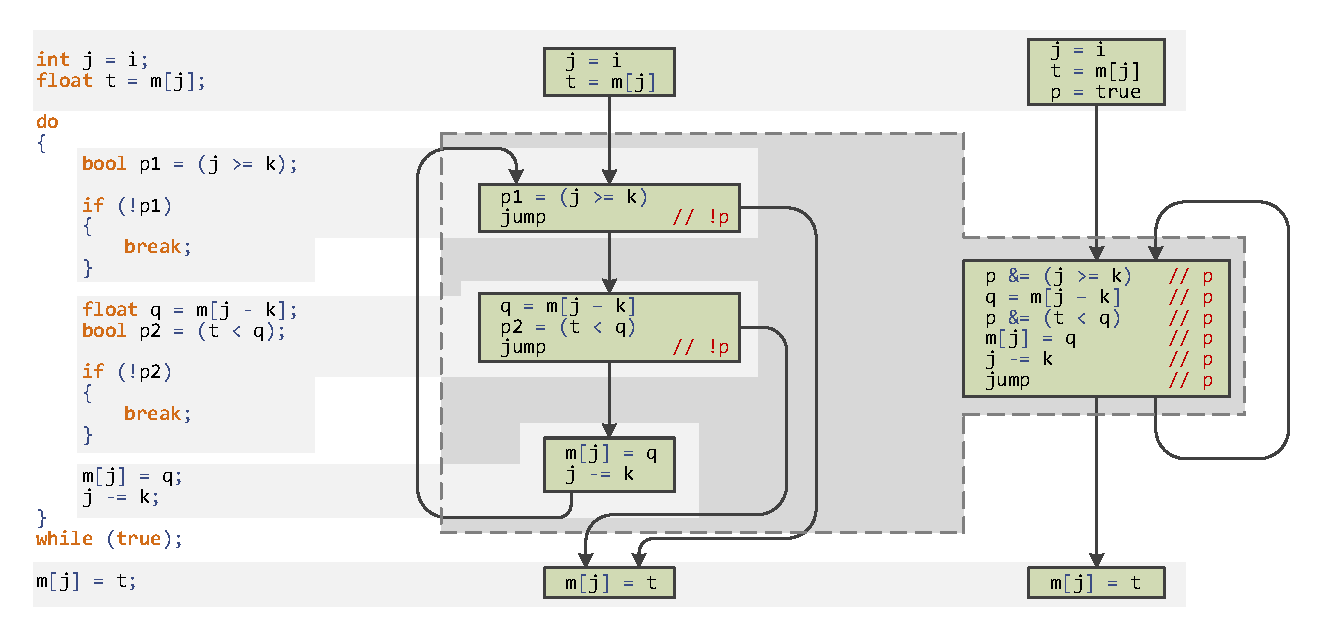
\includegraphics[width=1.0\textwidth]{./pics/text_4_vec_irreg/shell_cfg.pdf}
	\caption{}
	\label{fig:text_4_vec_irreg_shell_cfg}
\end{figure}

\begin{figure}[ht]
	\centering
		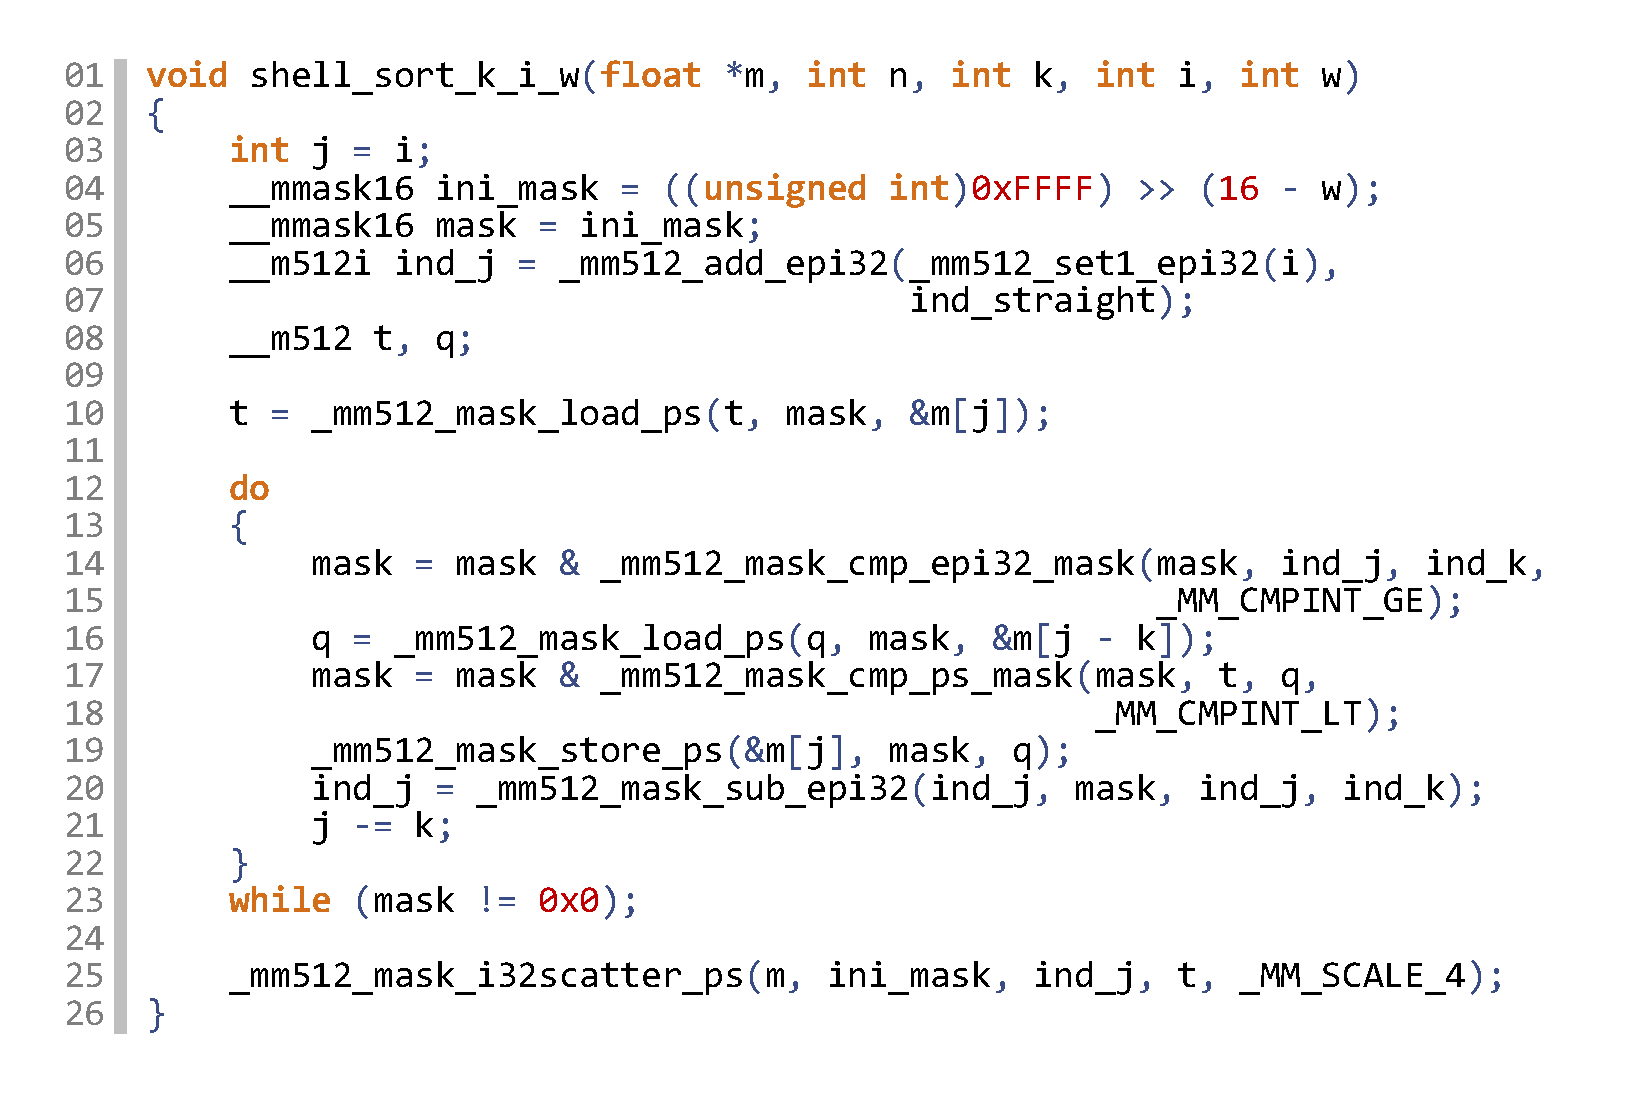
\includegraphics[width=0.8\textwidth]{./pics/text_4_vec_irreg/shell_code_vec.pdf}
	\caption{}
	\label{fig:text_4_vec_irreg_shell_code_vec}
\end{figure}

\begin{figure}[ht]
	\centering
		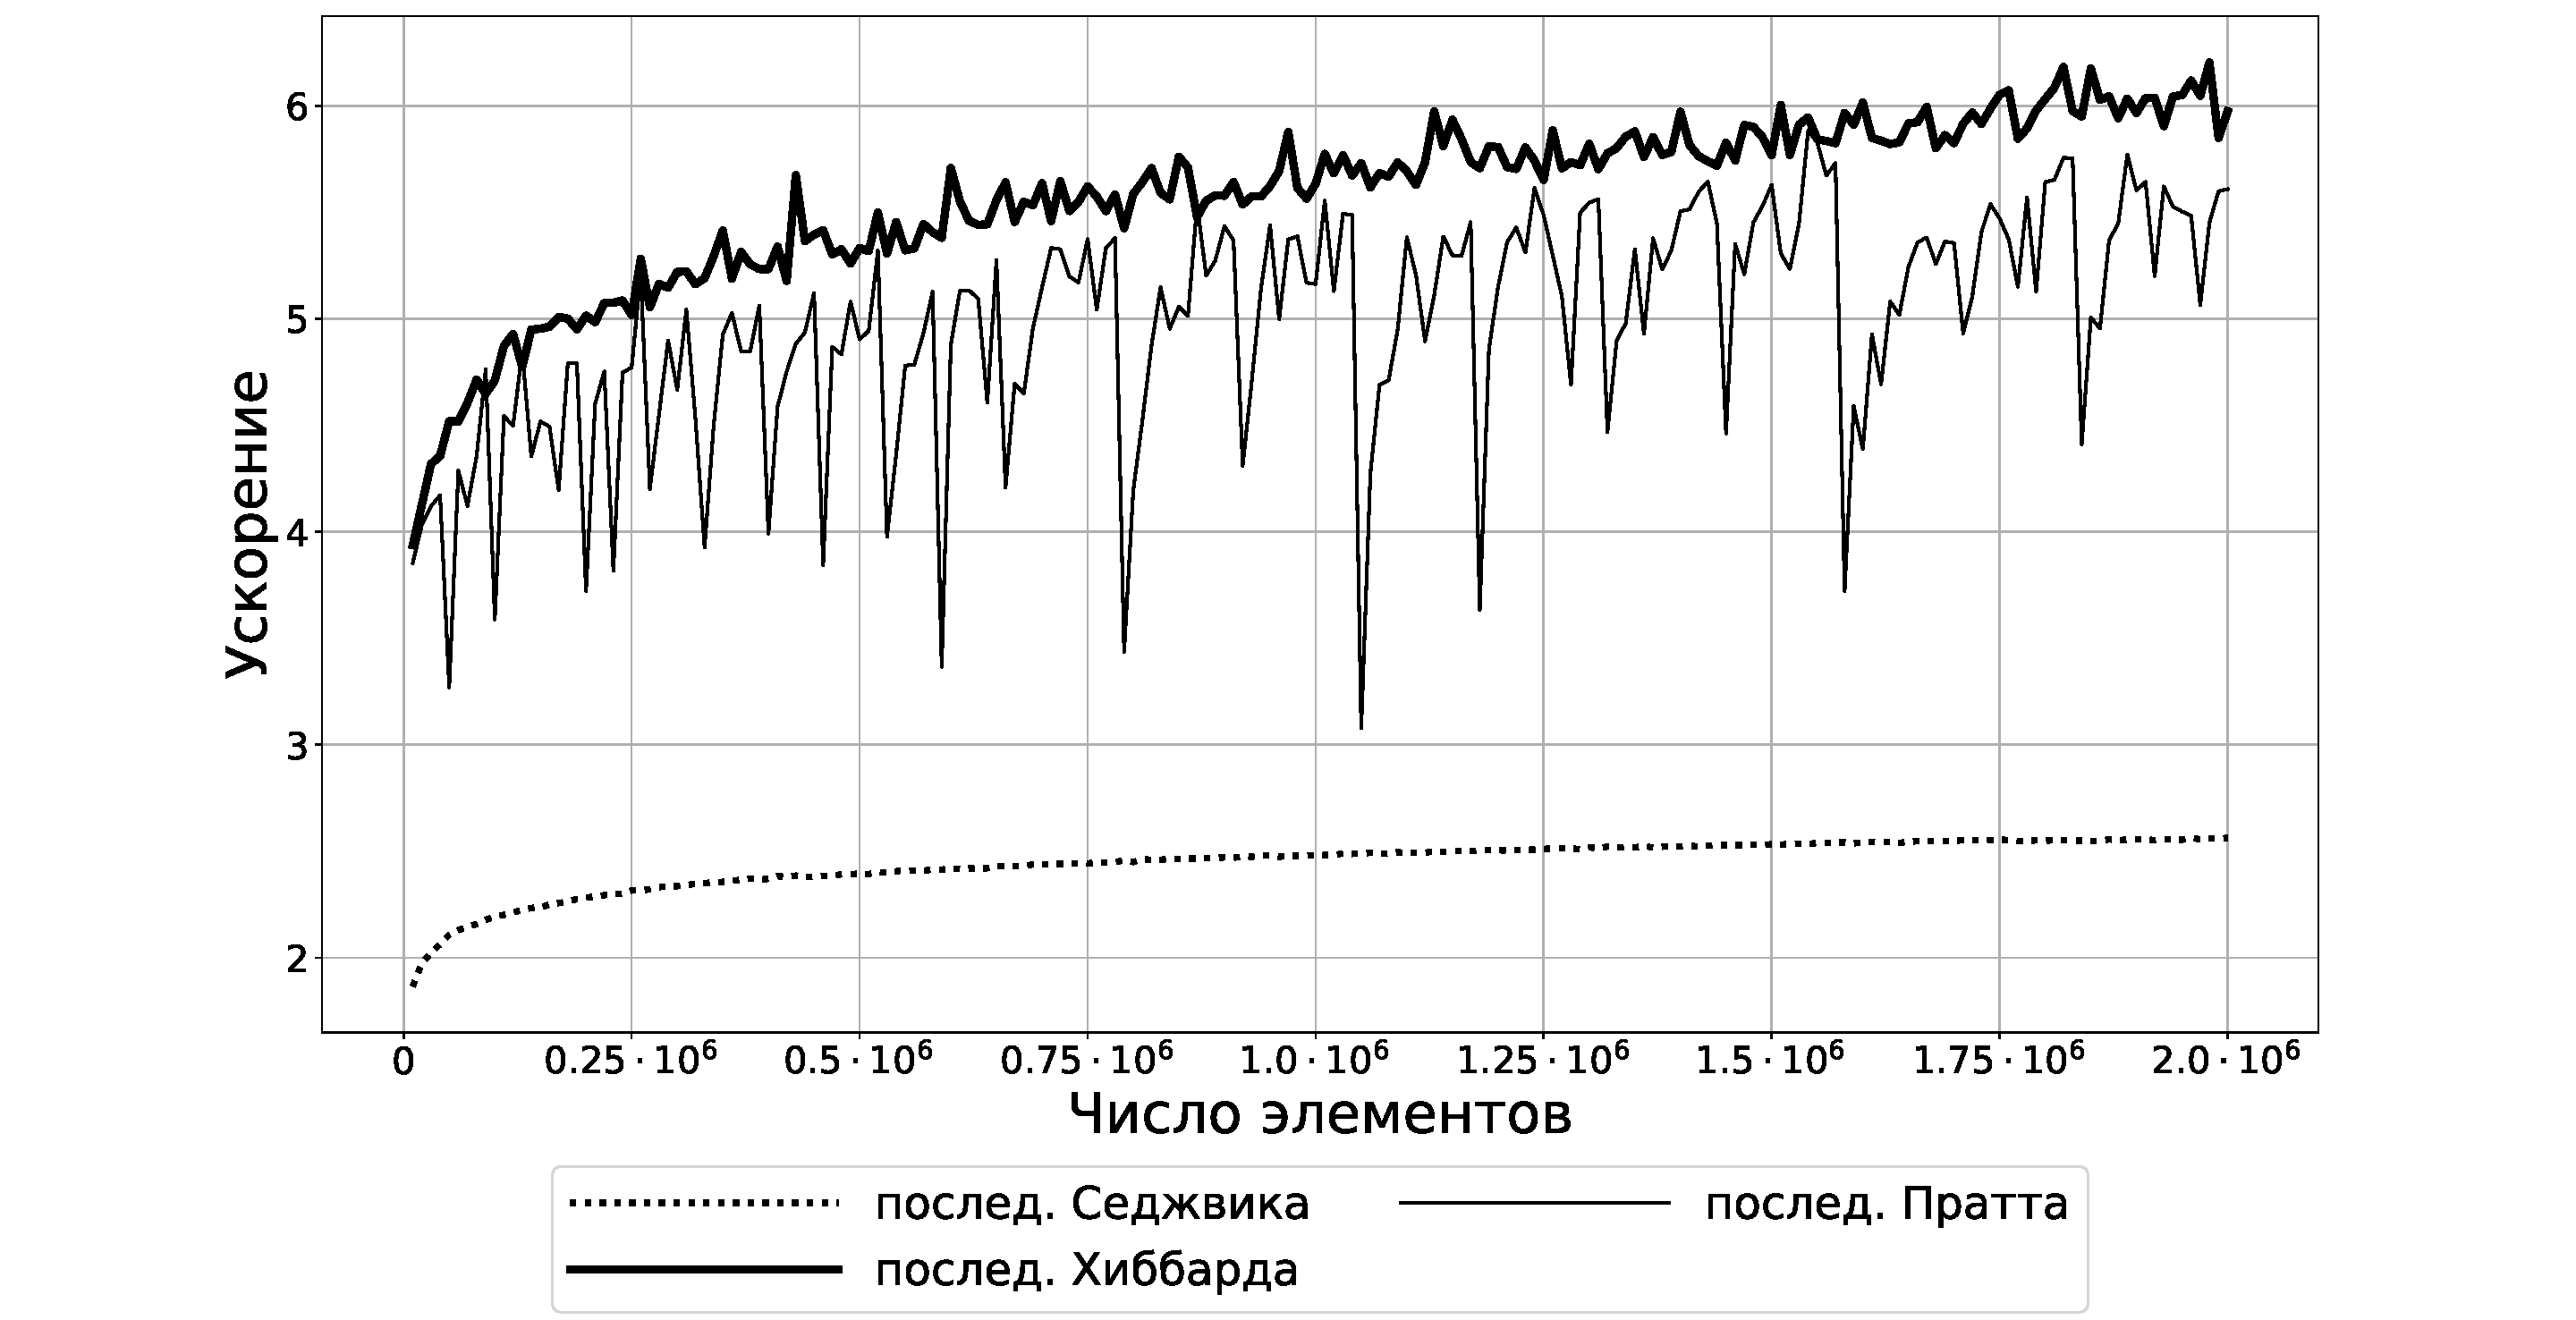
\includegraphics[width=1.0\textwidth]{./pics/text_4_vec_irreg/theoretical_eff.pdf}
	\caption{}
	\label{fig:text_4_vec_irreg_theoretical_eff}
\end{figure}

\begin{figure}[ht]
	\centering
		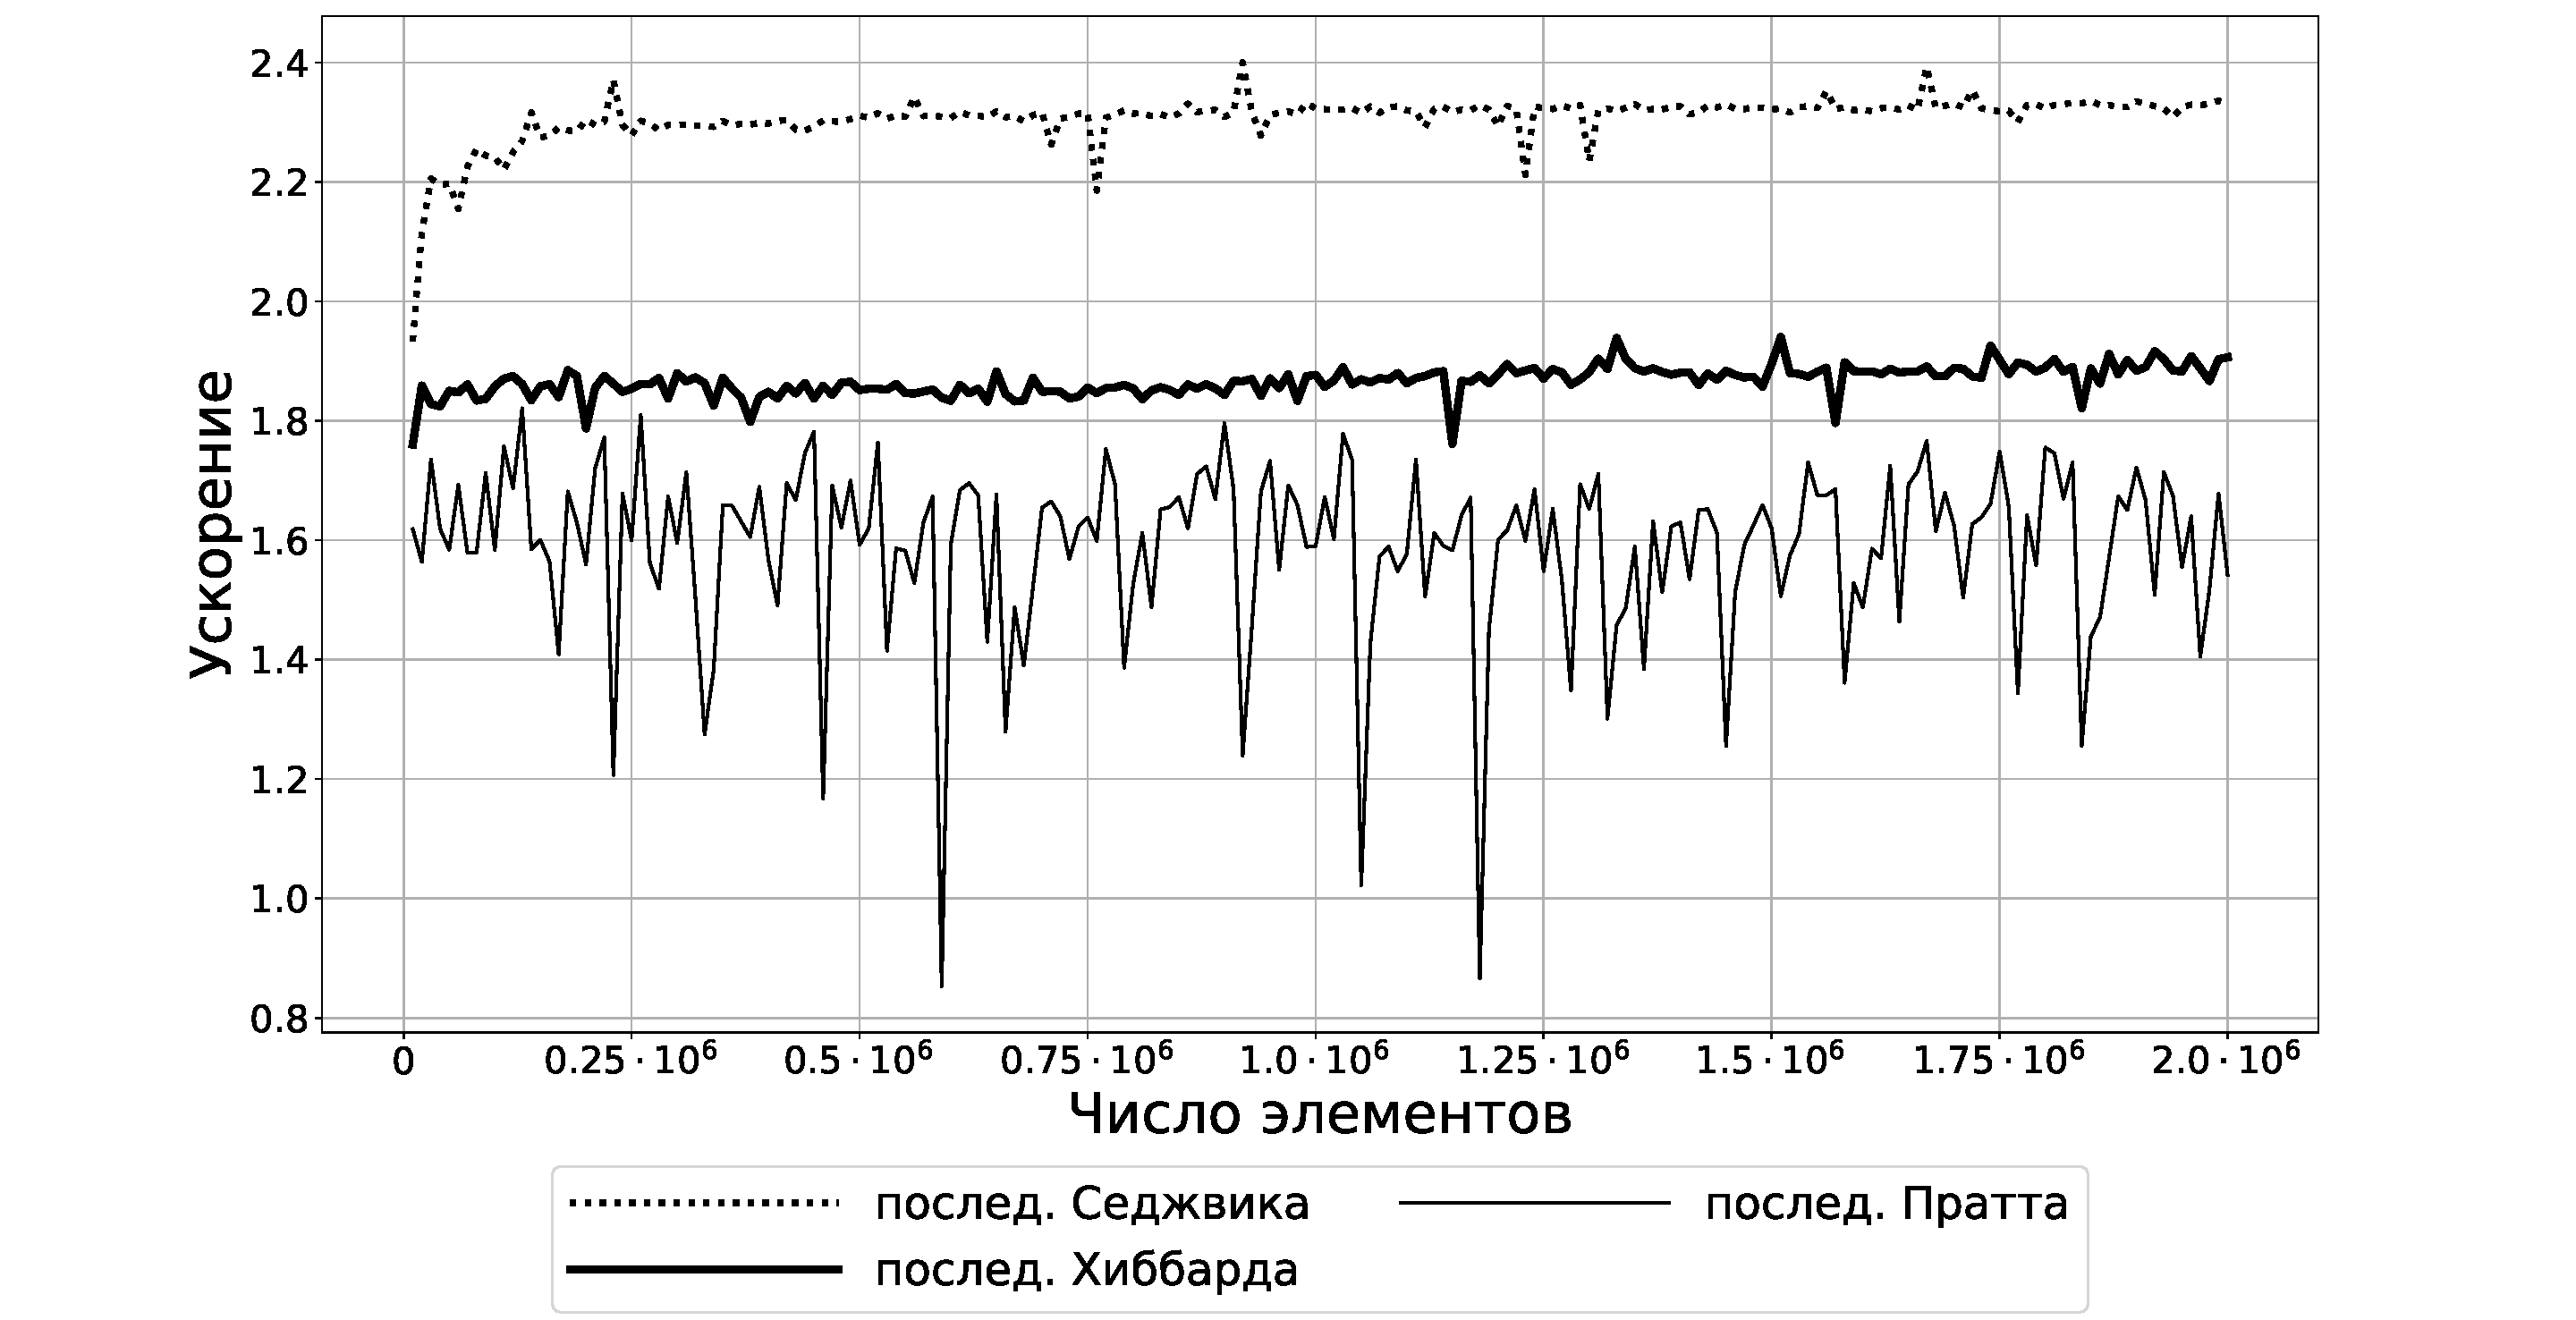
\includegraphics[width=1.0\textwidth]{./pics/text_4_vec_irreg/experimental_eff.pdf}
	\caption{}
	\label{fig:text_4_vec_irreg_experimental_eff}
\end{figure}

\begin{figure}[ht]
	\centering
		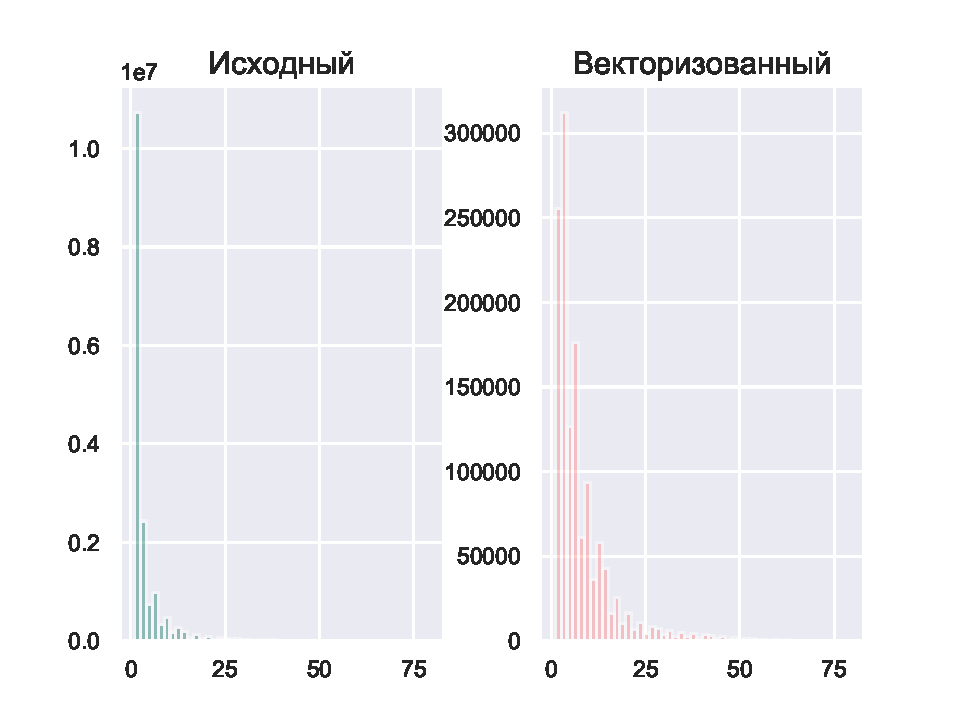
\includegraphics[width=0.8\textwidth]{./pics/text_4_vec_irreg/shell_k_4.pdf}
	\caption{}
	\label{fig:text_4_vec_irreg_shell_k_4}
\end{figure}

\begin{figure}[ht]
	\centering
		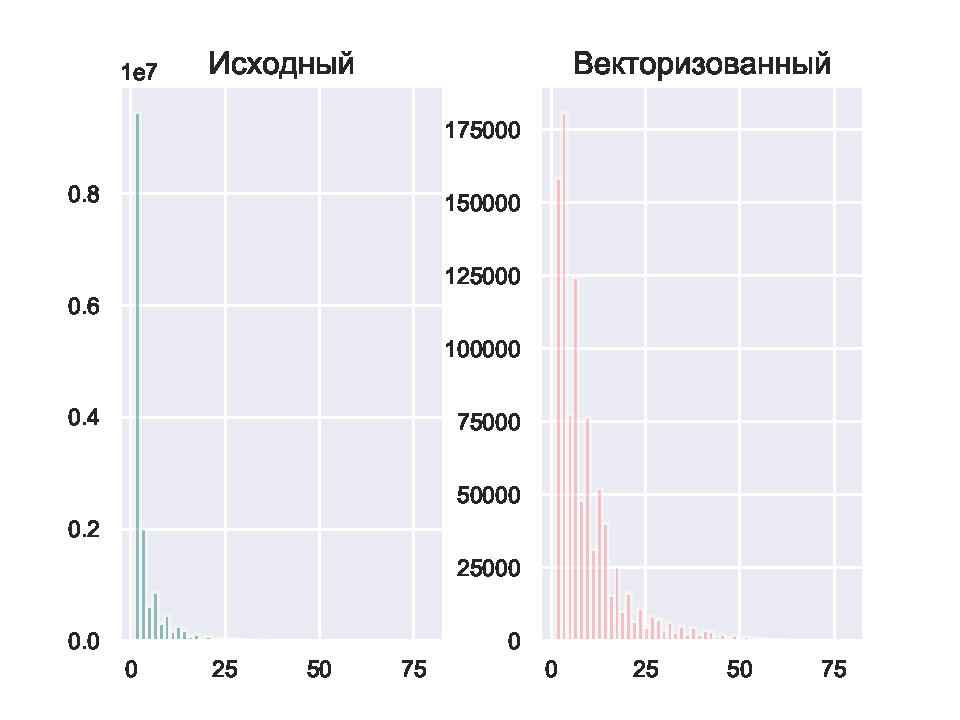
\includegraphics[width=0.8\textwidth]{./pics/text_4_vec_irreg/shell_k_15.pdf}
	\caption{}
	\label{fig:text_4_vec_irreg_shell_k_15}
\end{figure}

\begin{figure}[ht]
	\centering
		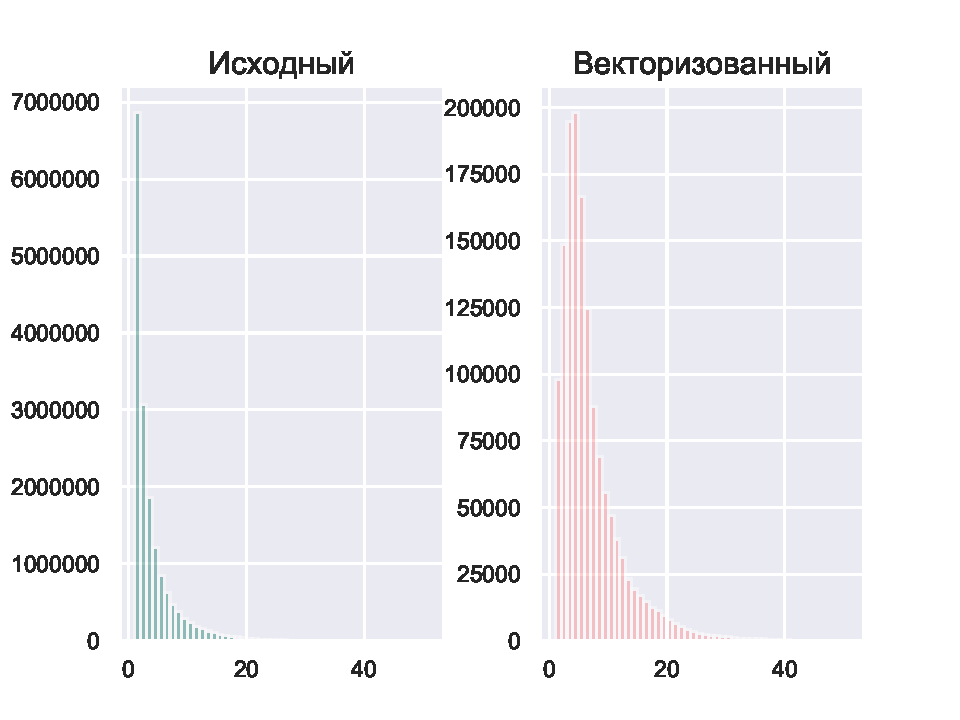
\includegraphics[width=0.8\textwidth]{./pics/text_4_vec_irreg/hibbard_k_3.pdf}
	\caption{}
	\label{fig:text_4_vec_irreg_hibbard_k_3}
\end{figure}

\begin{figure}[ht]
	\centering
		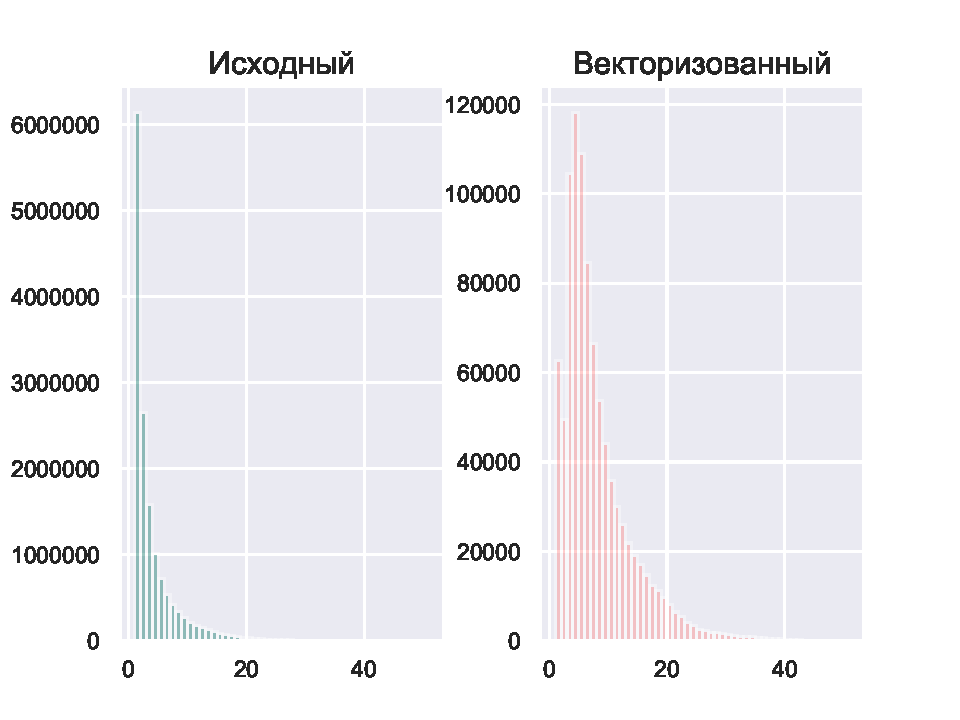
\includegraphics[width=0.8\textwidth]{./pics/text_4_vec_irreg/hibbard_k_15.pdf}
	\caption{}
	\label{fig:text_4_vec_irreg_hibbard_k_15}
\end{figure}
